%%%%%%%%%%%%%%%%%%%%%%%%%%%%%%%%%%%%%%%%%%%%%%%%%%%%%%%%%%%%%%%%%%%%%%%%%%%%%%%%
%2345678901234567890123456789012345678901234567890123456789012345678901234567890
%        1         2         3         4         5         6         7         8

\documentclass[letterpaper, 10 pt, conference]{ieeeconf}  % Comment this line out if you need a4paper

%\documentclass[a4paper, 10pt, conference]{ieeeconf}      % Use this line for a4 paper

\IEEEoverridecommandlockouts                              % This command is only needed if 
                                                          % you want to use the \thanks command

\overrideIEEEmargins                                      % Needed to meet printer requirements.

% See the \addtolength command later in the file to balance the column lengths
% on the last page of the document

% The following packages can be found on http:\\www.ctan.org
\usepackage{graphicx} % for pdf, bitmapped graphics files
%\usepackage{epsfig} % for postscript graphics files
%\usepackage{mathptmx} % assumes new font selection scheme installed
%\usepackage{times} % assumes new font selection scheme installed
\usepackage{amsmath} % assumes amsmath package installed
\usepackage{amssymb}  % assumes amsmath package installed

\usepackage{subfigure}

\title{Encounter Based Multi Robot Simultaneous Localization and Occupancy Grid Mapping}


% author names and affiliations
% use a multiple column layout for up to three different
% affiliations
\author{RB Choroszucha$^{1}$, C Hyman$^{2}$, and A Collier$^{3}$ % <-this % stops a space
\thanks{$^{1}$ RB Choroszucha is with the School of Naval Architecture and Marine Engineering, University of Michigan.  E-mail: riboch{@}umich.edu}%
\thanks{$^{2}$ C Hyman is with the School of Electrical Engineering and Computer Science, University of Michigan. E-mail: {hymanc}{@}umich.edu}
\thanks{$^{3}$ A Collier is with the School of Electrical Engineering and Computer Science, University of Michigan. E-mail: {amcollie}{@}umich.edu}
}



\begin{document}



\maketitle
\thispagestyle{empty}
\pagestyle{empty}


%%%%%%%%%%%%%%%%%%%%%%%%%%%%%%%%%%%%%%%%%%%%%%%%%%%%%%%%%%%%%%%%%%%%%%%%%%%%%%%%
\begin{abstract}

In this paper we present and implement the algorithm in Howard's 2006 paper: ``Multi-robot simultaneous localization and mapping using particle filters.''  We also make a small modification to allow for each robot to have its own particle filter and qualitatively demonstrate that it performs better than the current state of the art.


\end{abstract}

\section{Introduction}
\label{S:Intro}


The automated exploration of unknown environments has become one of the foremost challenges in mobile robotics. For a robot to explore an environment, it must map the environment and concurrently localize itself within the environment.  The framework used to perform this task is known as simultaneous localization and mapping (SLAM) and has been well covered in the literature using a variety of techniques \cite{durrant2006simultaneous,bailey2006simultaneous}.

While SLAM is well known and has a rich history of successes using a single robot, it can often be a slow process due to both constraints on the robot, such as speed and data processing, and lack of redundancy, i.e. robot failure \cite{thrun2001probabilistic,burgard2005coordinated}.  To address the speed of mapping and to add redundancy, coordinated or multi-robot SLAM (MRSLAM) was created.

MRSLAM is as it sounds, SLAM using multiple exploring robots. This approach allows for the partition of the physical search space using different robots, typically decreasing the time it takes to map an area, and increasing the likelihood of full map coverage in the event of robot failure. This temporal exploration parallelism does, however, come at the cost of added complexity. The added complexity of MRSLAM comes in two major components: coordination of exploration using multiple search agents and merging the maps of these agents \cite{fox2006distributed}.  Coordinated exploration consists of planning the groups' search path, most often formulated to cover the most search space in minimum time or to optimize some other mapping cost criteria. The other major component, map merging, is the combination of individual robot's observations and maps into one cohesive global map estimate.

In this paper we use the map merging algorithm presented in Howard's 2006 paper: ``Multi-Robot Simultaneous Localization and Mapping using Particle Filters'' \cite{howard2006multi} to build an occupancy grid of a defined space. This paper is of particular interest as it presents a resource efficient online solution to the MRSLAM map merging problem given unknown initial robot poses.  

The algorithm presented is an encounter-based algorithm.  Given that we start with one mapping robot (call this Robot 1), when it encounters another robot (Robot 2), the relative pose between the two robots is computed and Robot 2's odometry and scan data is transmitted in reverse order to Robot 1, where the data is integrated to create a single map posterior.

Fig. \ref{fig:HowardFig3} depicts the process with robot 1's Pose-Actuator-Sensor triple $(x^1_t,u^1_{t-1},z^1_t)$ (PAS triple), and robot 2's PAS triple $(x^2_t,u^2_{t-1},z^2_t)$.
When $t=2$, robot 1 observes robot 2 and determines the relative pose $\Delta$, then the past odometry and scan data is integrated in reverse order.

\begin{figure}[h]
\centering
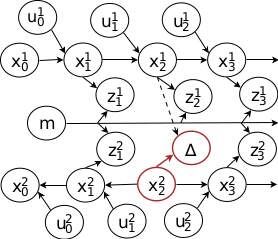
\includegraphics[width=\columnwidth]{{{../FinalFigures/HowardFig3}}}
\caption{Depiction of data integration. Taken from \cite{howard2006multi}.}
\label{fig:HowardFig3}
\end{figure}

The paper is structured as follows: In \S\ref{S:Back} some background about MRSLAM is provided, the contribution of \cite{howard2006multi} and the modified algorithm is discussed .  In \S\ref{S:Alg} the algorithm of \cite{howard2006multi}, and its modification, is presented.  In \S\ref{S:Exp}, the two algorithms are compared qualitatively using a simulated data set. 




\section{Background}
\label{S:Back}

\subsection{State of the Art}
\label{SS:Back:SOA}
    
In the literature there are two problems that are often addressed when dealing with MRSLAM:
\begin{enumerate}
\item robot coordination, i.e., how to cover the most area given an unknown environment \cite{julia2012comparison}, and
\item merging the data to create one global map posterior, which is what we will focus on.
\end{enumerate}

In the case where all relative robot poses are known, merging maps is a trivial problem using small modifications to existing SLAM techniques \cite{thrun2001probabilistic}. In the general MRSLAM problem, however, robots may start with unknown absolute and relative poses, and therefore merging of maps requires the discovery of relative relationships between different robot trajectories to build a single map. This is often a costly process, which in general can be solved for robots sharing a search space by estimating each robot's relative pose given a partial map, but this leads to exponential complexity with respect to the number of exploring robots \cite{fox2006distributed}. Nevertheless, several practical algorithms exist to circumvent this naive and inefficient approach,  including coarse topological matching and stitching techniques borrowed from computer vision \cite{birk2006merging}.

To combat this a large majority of the MRSLAM papers employ a Rao-Blackwellized particle filter (RBPF) for building occupancy grids.


\cite{howard2006multi,birk2006merging,lazaro2013multi,lee2012probabilistic}


-Where did it begin, what did it progress to?




\subsection{\cite{howard2006multi} Extension to Original Work}
\label{SS:Back:Contributions}


Define the weights for a particle filter: $w_t^i$, and the sensor model, $p(z_t|x_t,u_{t-1})$ for the forward and reverse model.  In \cite{howard2006multi}, Howard follows the typical RBPF formulation and defines the un-normalized weight update to be:
\begin{equation}
w^i_t=p(z_{t,f}|x_{t,f}^i,m_{t-1,f}^i) p(z_{t,r}|x_{t,r}^i,m_{t-1,r}^i) w^i_{t-1}.
\label{eq:combinedweight}
\end{equation}

In this formulation it is no stretch of the imagination that the highest weight $p(z_{t,f}|x_{t,f}^i,m_{t-1,f}^i) w^i_{t-1}$ can be quite large, denoting a good match to the data in the forward direction, yet the reverse direction sensor model, $p(z_{t,r}|x_{t,r}^i,m_{t-1,r}^i)$, could be small.  Thereby reducing the probability that the best forward direction


In this work, we propose assuming that forward and reverse motions are independent, resulting in two particle filters with weights defined by:
\begin{eqnarray}
w^i_{t,f}&=&p(z_{t,f}|x_{t,f}^i,m_{t-1}^i)  w^i_{t-1,f}\\
w^i_{t,r}&=&p(z_{t,r}|x_{t,r}^i,m_{t-1}^i)  w^i_{t-1,r}
\end{eqnarray}
and with $\{x_{t,f}^i,m_{t-1}^i\}$ being resampled using $\{w^i_{t,f}\}$, and $\{x_{t,r}^i\}$ being resampled using $\{w^i_{t,r}\}$.  

Fig. \ref{fig:deplete} is an example where the best forward and backward particles would be chosen independently; however, when the weights are combined as in \eqref{eq:combinedweight}, we see case where the best forward or reverse particles (e.g, particle 1) will mostly likely not be resampled.

\begin{figure}[h]
\centering
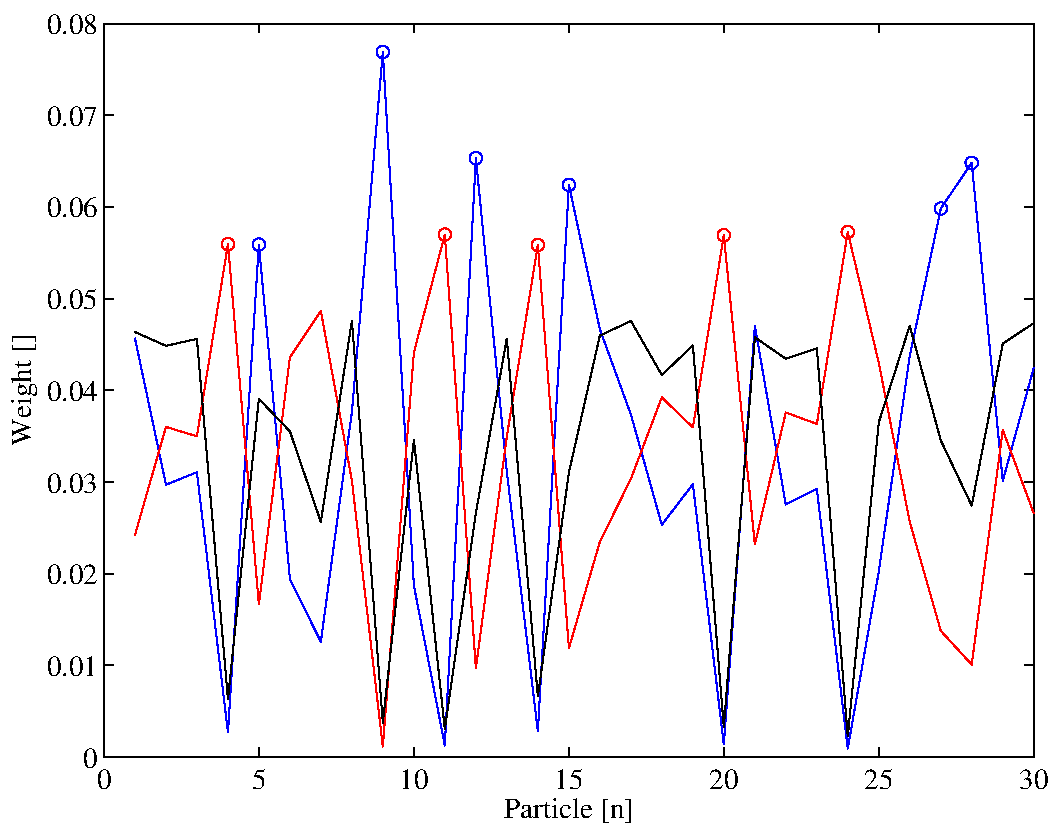
\includegraphics[width=\columnwidth]{../FinalFigures/Depletion}
\caption{Case where the best forward and reverse poses are not chosen. $w^i_{t,f}$ is the forward weight, $w^i_{t,r}$ is the reverse weight, and $w^i_t$ is the product of the weights.}
\label{fig:deplete}
\end{figure}

The contribution is two-fold, verifying that Howard's algorithm works, and creating a independent particle filters for each mapping robot in the aim to build a better occupancy grid, and obtain a better localization within the map.



\section{The Algorithm}
\label{S:Alg}

\subsection{Overview}
\label{SS:Alg:Overview} 


Howard’s multi-robot SLAM algorithm generates a single map and pose posterior much in the same way an occupancy grid map SLAM algorithm based on a Rao-Blackwellized particle filter (RBPF) would, but with additions to accommodate multiple robots. Mapping begins with a set consisting of a single robot with known pose and an occupancy grid map of the environment is built as this robot traverses and measures it. The ultimate goal of the algorithm is to simultaneously compute for time $t$, the full SLAM posterior containing all robot pose trajectories $x_{1:t}^i$ and the global map $m_{1:t}$, given only a single known initial pose and sets of measurements
$$p(x_{1:t}^1,x_{1:t}^2,...,x_{1:t}^M,m_{1:t}|x_0^1,z_{1:t}^1,u_{0:t}^1,\Delta_s^2,z_{1:t}^2,u_{0:t}^2,\Delta_s^3,...,\Delta_s^M,z_{1:t}^M,u_{0:t}^M)$$

The odometry and measurement data of all other robots is stored as it is collected, as it cannot contribute to the global map without a known relative pose linking it to the frame of the first robot. As the first robot encounters additional robots via a mutual pose observation, the newly observed robot is added to the set of mapping robots and its actions and the map is sequentially conditioned by its actions and measurements. From the point of observation, all future actions and measurements of the new robot are used to condition the map posterior, and likewise all of its previously stored actions and measurements are played back in reverse order from that point as a virtual robot. This information is then passed to a pair of new particle filters for the pose of these robots that contribute to the same global map. 
As further encounters occur between any robot, real or virtual, in the mapping set and a previously unseen robot, the previously unseen robot is added to the set of mapping robots and its measured relative pose is again used to establish a reference point with which its actions and measurements can condition the map posterior. Further mutual observations of two robots already in the mapping set are ignored for the sake of simplicity. This encounter-add process is continued recursively for all robots until all stored and future odometry and measurements are exhausted or all possible mapping robots have made an encounter with the mapping set. Beyond this point, the algorithm behaves as a normal RBPF with a stacked state containing pose posteriors of all robots in addition to the map.


    This algorithm relies on a number of assumptions that are requisite for it to effectively solve the MRSLAM problem. Firstly, for all explored regions to count towards the map, each mapping robot must have encountered a robot that is an element of the mapping set in order to make a fully connected graph of robot poses, and therefore maximally complete map. Additionally, each robot pose trajectory is independent of all other trajectories such that motion or observation from one robot does not affect another outside of encounter events \cite{howard2006multi}.



\section{Experimental Validation}
\label{S:Exp}



\begin{figure*}[ht]
\centering
\subfigure[The test geometry, robot paths, and encounters (gray).]{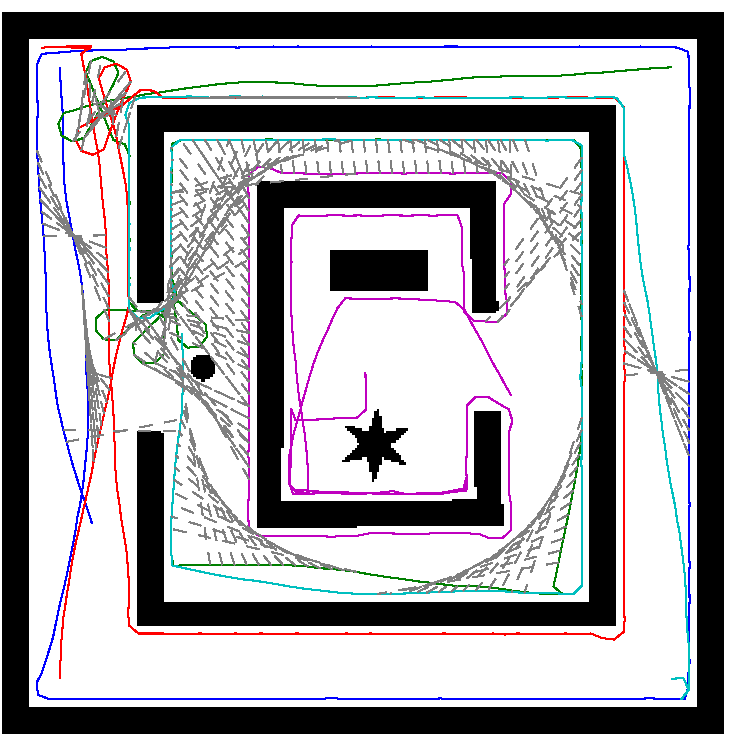
\includegraphics[width=\columnwidth]{../FinalFigures/Encounters}}
\subfigure[Robot encounters at a given time.]{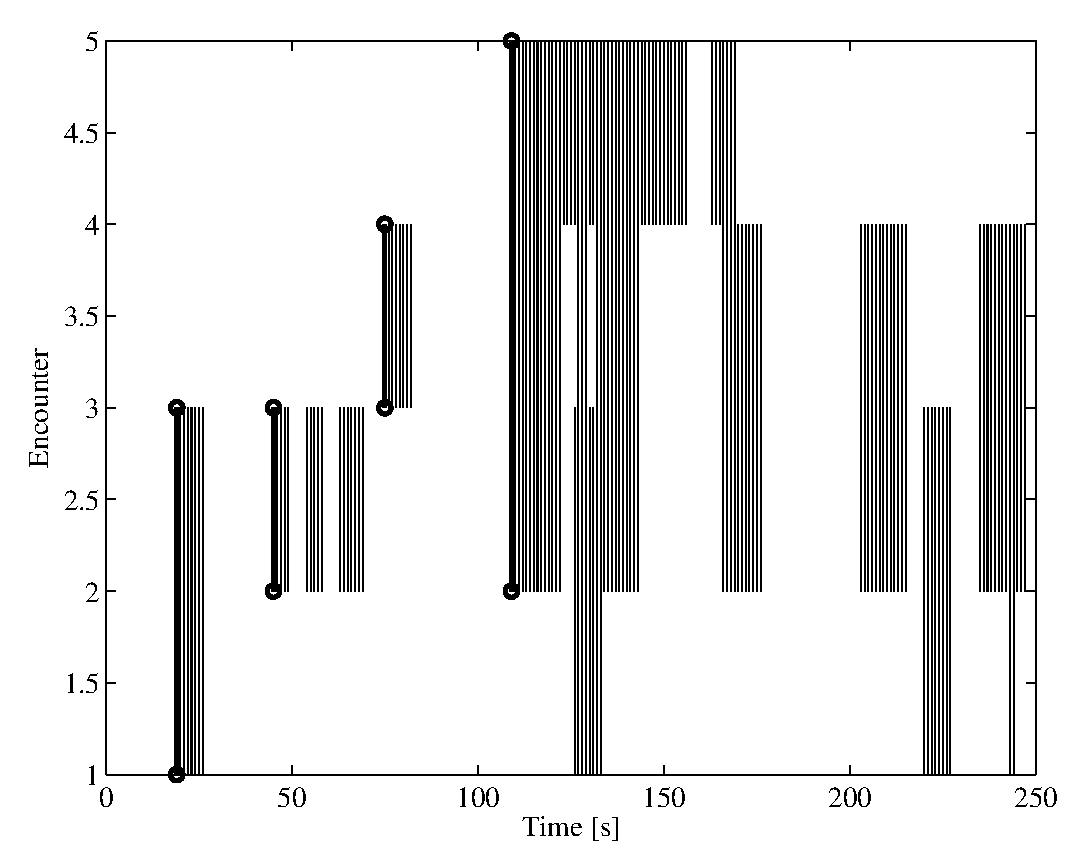
\includegraphics[width=\columnwidth]{../FinalFigures/EncountersTimes}}
\caption{}
\end{figure*}



\begin{equation}
\begin{bmatrix}
x_{t}\\
y_{t}
\theta_{t}
\end{bmatrix}=\begin{bmatrix}
x_{t-1}\\
y_{t-1}
\theta_{t-1}
\end{bmatrix}+\begin{bmatrix}
dx_t \cos(\theta_t+d\theta_t)\\
dy_{t}\sin(\theta_t+d\theta_t)\\
\theta_{t-1}+d\theta_t
\end{bmatrix}
\label{eq:OdometryMotion}
\end{equation}

\begin{figure}[ht]
\centering
\subfigure[Known Poses]{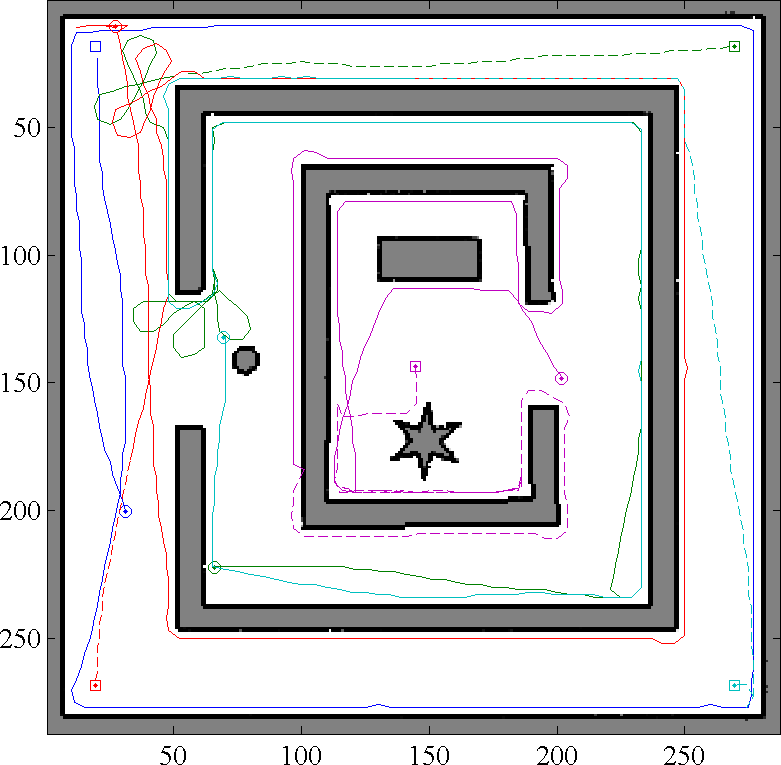
\includegraphics[width=\columnwidth]{../FinalFigures/KnownPoses}}
\subfigure[Pure Odometry]{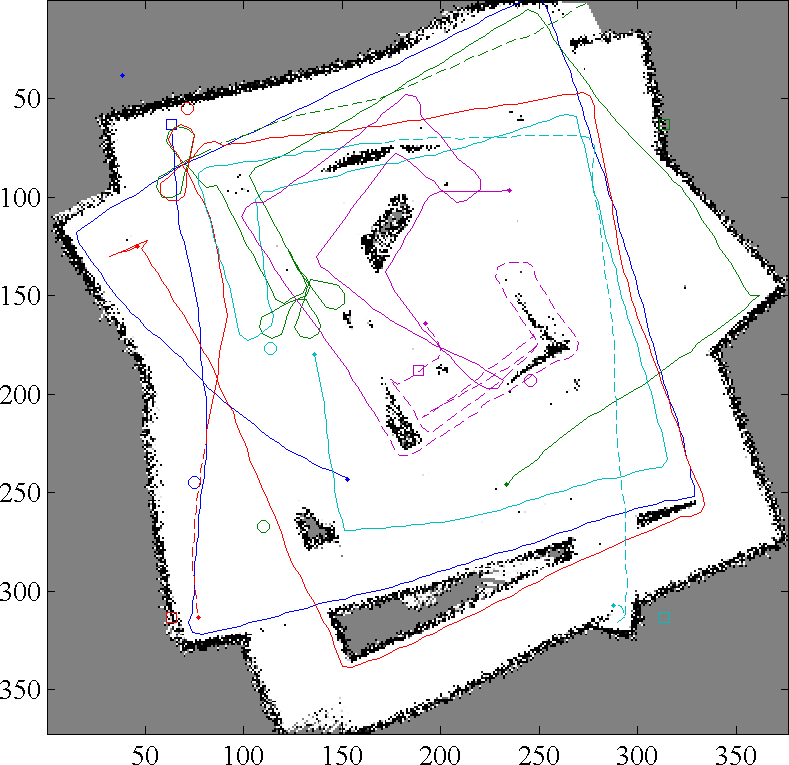
\includegraphics[width=\columnwidth]{../FinalFigures/PureOdometry}}\\
\subfigure[Howard Implementation: Unknown Poses, low noise.]{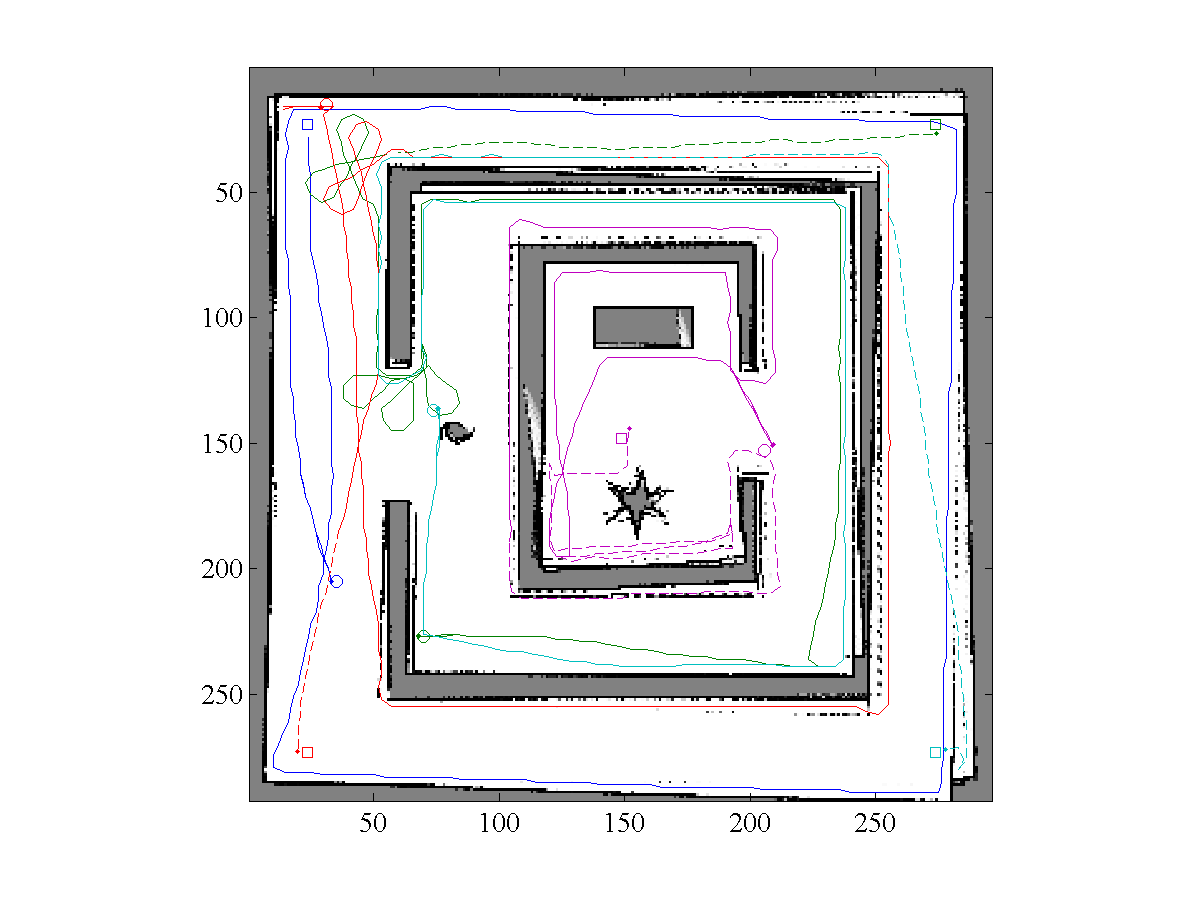
\includegraphics[width=\columnwidth]{../FinalFigures/HowardLowNoise}}
\subfigure[Proposed Implementation: Unknown Poses, low noise.]{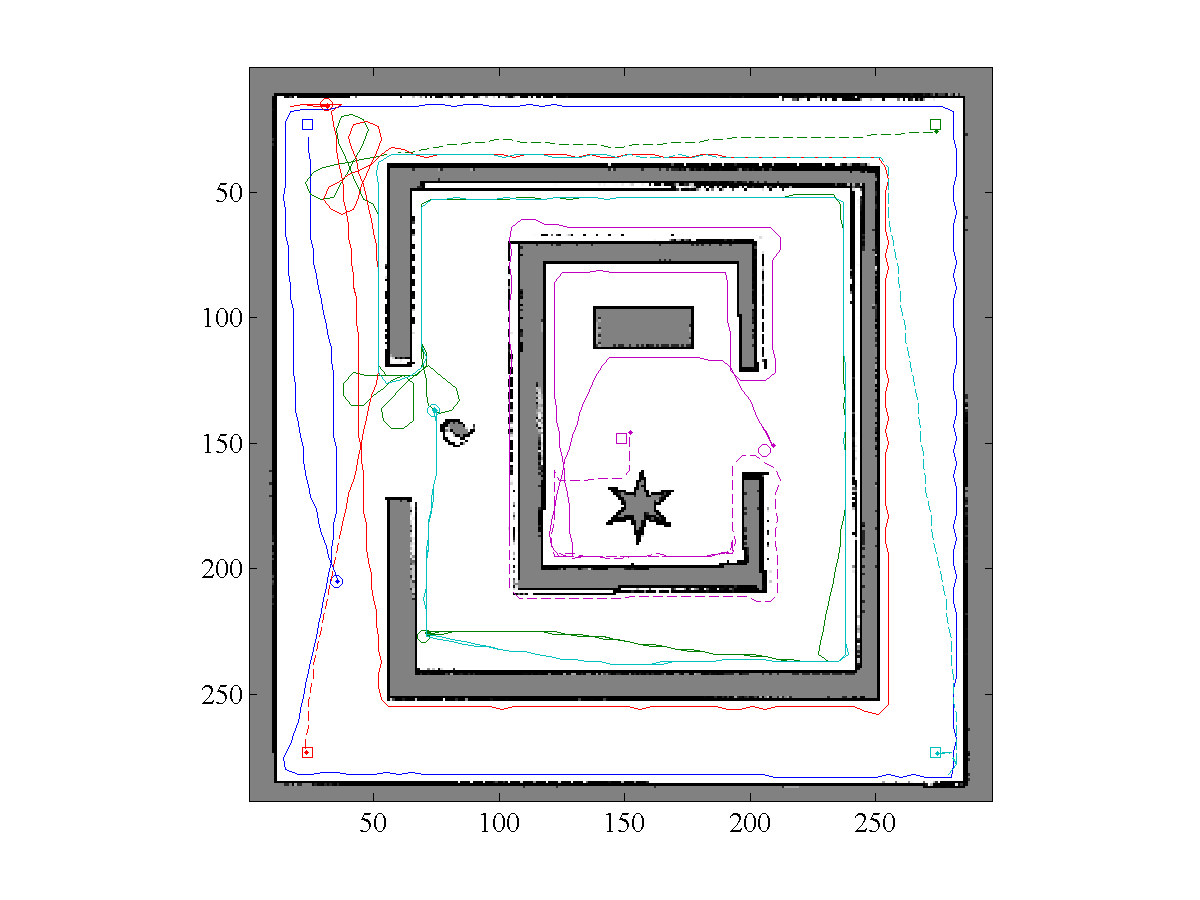
\includegraphics[width=\columnwidth]{../FinalFigures/OursLowNoise}}\\
\subfigure[Howard Implementation: Unknown Poses, High noise.]{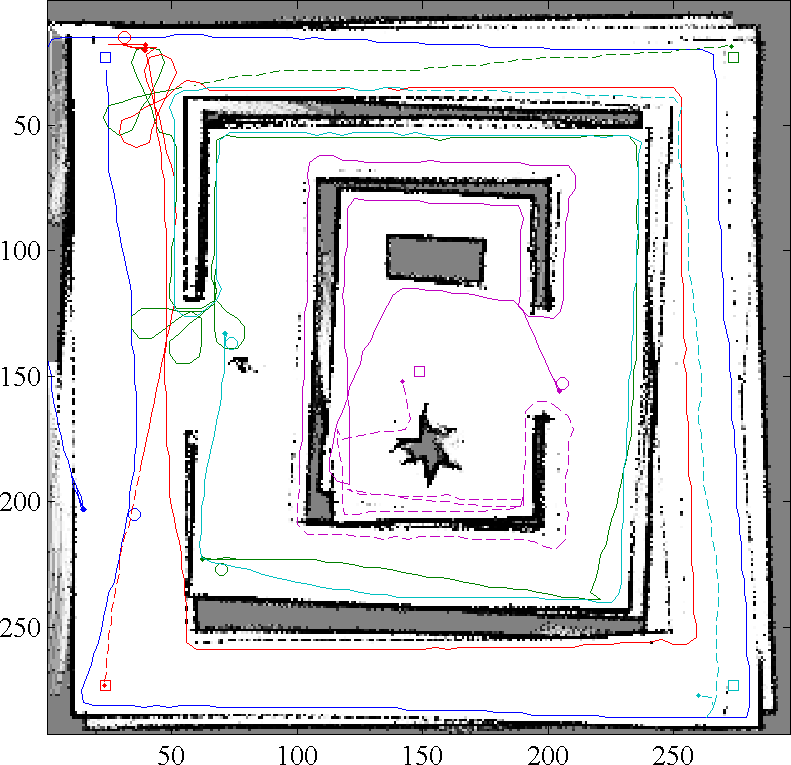
\includegraphics[width=\columnwidth]{../FinalFigures/HowardHighNoise}}
\subfigure[Proposed Implementation: Unknown Poses, High noise.]{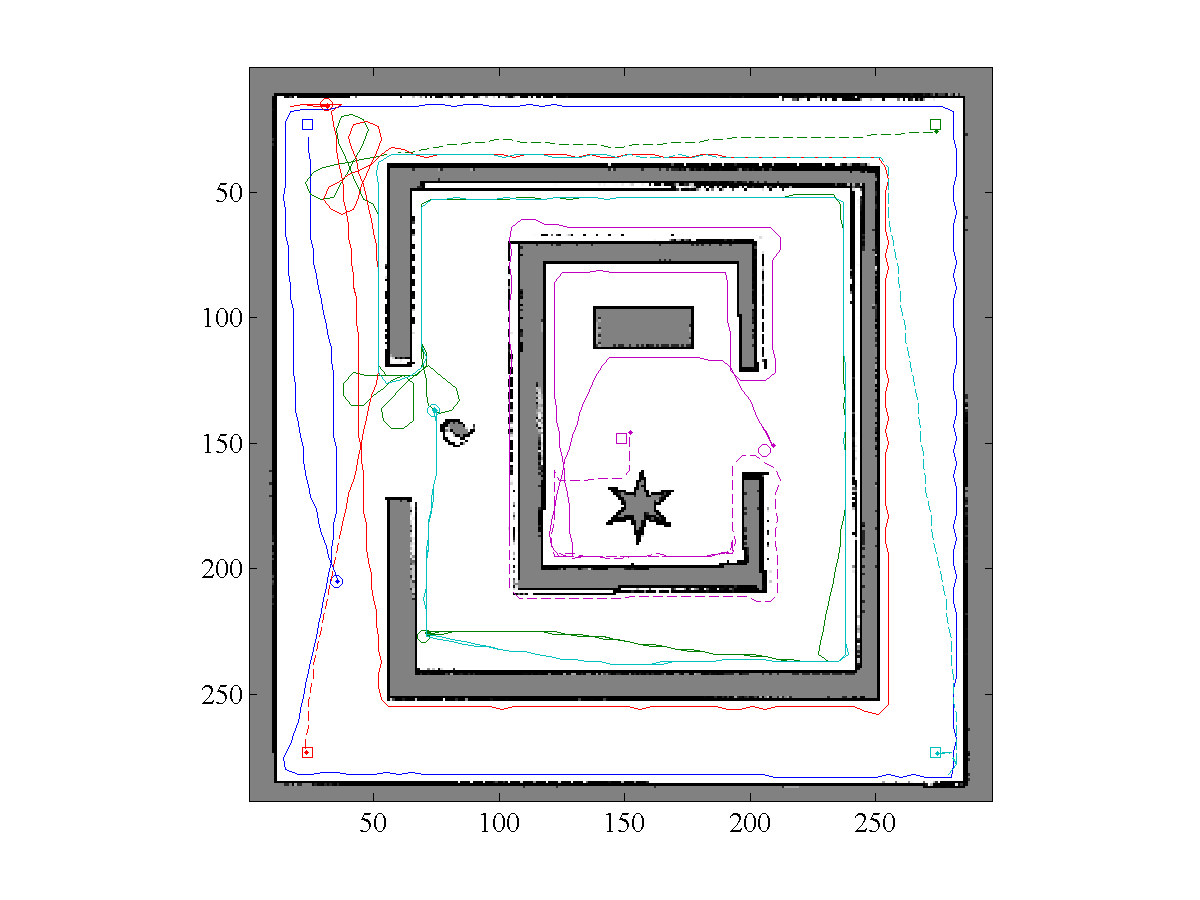
\includegraphics[width=\columnwidth]{../FinalFigures/OursLowNoise}}
\caption{Comparison between Howard's implementation and the proposed implementation.}
\end{figure}




\section{Conclusion}


\bibliographystyle{plain}
\bibliography{Citations}

%%%%%%%%%%%%%%%%%%%%%%%%%%%%%%%%%%%%%%%%%%%%%%%%%%%%%%%%%%%%%%%%%%%%%%%%%%%%%%%%
\addtolength{\textheight}{-12cm}   % This command serves to balance the column lengths
                                  % on the last page of the document manually. It shortens
                                  % the textheight of the last page by a suitable amount.
                                  % This command does not take effect until the next page
                                  % so it should come on the page before the last. Make
                                  % sure that you do not shorten the textheight too much.

%%%%%%%%%%%%%%%%%%%%%%%%%%%%%%%%%%%%%%%%%%%%%%%%%%%%%%%%%%%%%%%%%%%%%%%%%%%%%%%%



%%%%%%%%%%%%%%%%%%%%%%%%%%%%%%%%%%%%%%%%%%%%%%%%%%%%%%%%%%%%%%%%%%%%%%%%%%%%%%%%



%%%%%%%%%%%%%%%%%%%%%%%%%%%%%%%%%%%%%%%%%%%%%%%%%%%%%%%%%%%%%%%%%%%%%%%%%%%%%%%%





\end{document}
